\section{Experiments}
In this section, we assess the performance of PSRs and different kinds of Multi-PSRs. We do so over many different configurations of parameters, the most relevant ones being the model size, the number of observations used, and the type of environment. For all the plots, the x-axis is model size of the PSR/M-PSRs and the y-axis is an error measurement of the learned PSR/M-PSRs.

\subsection{Obtaining Observation Sequences}
In all the experiments, an agent is positioned in a starting location and stochastically navigates the environment based on a transition function $\delta:S \times S\rightarrow[0,1]$. Whenever a transition occurs an observation symbol is produced. When the agent exits the labyrinth, we say the trajectory is finished, and we record the concatenation of the symbols produced. We call this concatenation the observation sequence for that trajectory.  

\subsection{Learning Implementation: Timing v.s Multiple Symbols}

For the timing case, we construct our empirical hankel matrix by taking P,S = $\{a^i, \forall i<=n\}$. The parameter n depends on the application. For Double Loop environments we set $n = 150$, while for the pacman labyrinth $n = 600$. For these choices of n, we verify that as the amount of data gets large the learned PSR with the true model size becomes increasingly close to the true model. For Base M-PSR, we set $b=2,K=9$, so that the longest string in $\Sigma'$ is $a^{256}$.

For multiple observations a slightly more complex approach is required to choose P and S. For prefixes P, we select the k most frequent prefixes from our observation set. For suffixes S, we take all suffixes that occur from P. We also require prefix completeness. That is, if p' is a prefix of p $\in P$, then p' $\in P$. This heuristic for constructing empirical hankel matrices was given in previous work by [] and it showed that (). For the Base M-PSR, we take K=8 and B=2 for both symbols $\Sigma=\{g,b\}$, g for green and b for blue. For the Tree M-PSR we set $L=7$ for a total of 128 operators, a far larger allowance than the other M-PSRs. 

\lucas{Borja's heuristics for choosing P,S need citation and explanation}

\subsection{Measuring Performance}

To measure the performance of a PSR/M-PSR we use the following norm:
\begin{equation*}
||f - \hat{f}|| = \sqrt{\sum\nolimits_{x \in observations}(f(x) - \hat{f(x)})^2}
\end{equation*}
We use this norm because of a bound presented by [AUTHORS], which states that (). Here the function f denotes the true probability distribution over observations and the function $\hat{f}$ denotes the function associated with the learned M-PSR/PSR. In our environments, the function f is obtainable directly as we have access to the underlying HMMs.

Since the set of observations $\Sigma^{\star}$ is infinite, we compute approximations to this error norm, by fixing a set of strings T and summing over T. For the timing case, we take $T = \{a^i, \forall i<=C\}$ with C=600. Importantly C large enough such that $\sum_{i=0}^{C}f(a^i)>0.99$. For the multiple observation case, we take all possible strings producible from the prefixes and suffixes in our dataset. That is, for the multiple observation case $T = \{ps, \forall p \in P, \forall s \in S\} $

\lucas{Need citation for bound on norm2 error}

\section{Double Loop Timing}

For timing, we start by considering a double loop environment. The lengths of the loops correspond to the number of states in the loop. A trajectory begins with the agent starting at the intersection of the two loops. Here, the agent has a 50\% probability of entering either loop. At intermediate states in the loops the agent moves to the next state in the loop with probability 1-P or remains in its current state with probability P. Here, P represents the self-transition probability for internal states. Exit states are located halfway between each loop. Agents leaving the environment at exit states with 50\% probability. This means that if loop lengths are $l_1=64$ and $l_2=16$, we observations will come in the form of $n_1*l_1+n_2*l_2+(1-\alpha)*l1_/2 + \alpha*l2/2$, with $\alpha=1$ representing an exit through loop1 and $\alpha=0$ an exit through loop2.

\subsection{Number of Trajectories}

Here, we vary the number of observations used in our dataset. PSRs/M-PSRs learned in Figure 1 use 100 observation sequences, while those in Figure 2 use 10000. In both cases the M-PSRs outperform the standard PSR for reduced model sizes.

\begin{figure}[ht!]
\centering
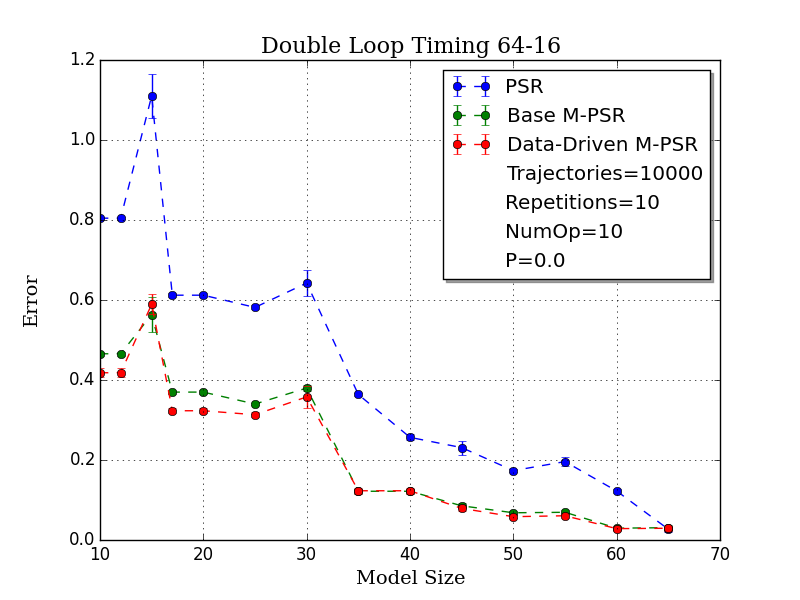
\includegraphics[width=60mm]{uCOREPICS/DL/64-16-10000.png}
\caption{Low Data Double Loop 64-16\label{overflow}}
\end{figure}

\begin{figure}[ht!]
\centering
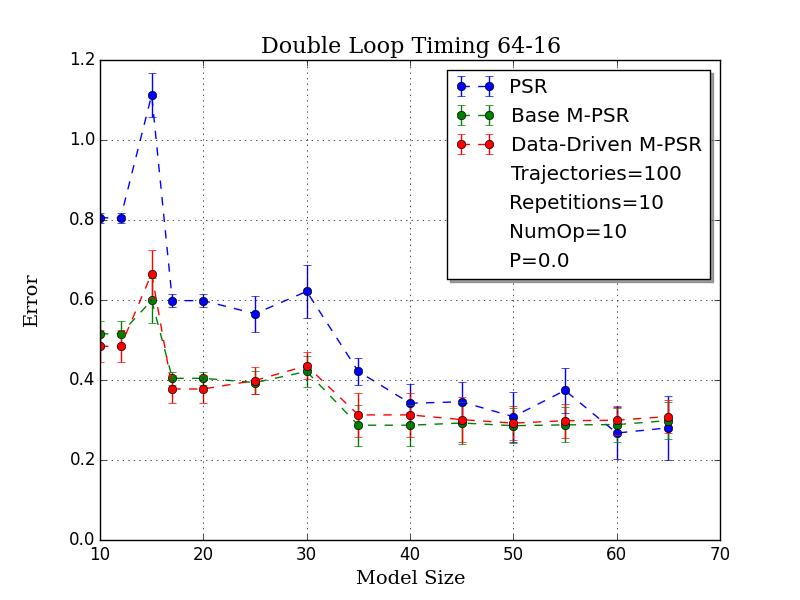
\includegraphics[width=60mm]{uCOREPICS/DL/64-16-100.png}
\caption{High Data Double Loop 64-16\label{overflow}}
\end{figure}

\subsection{Noise: P}

Next, we vary the self-transition probability P to simulate noise in an environment. Figure 3 is a 64-16 double loop with P=0.2, and Figure 1 is a 64-16 double loop with P=0. We find that the noisy loops are more compressible, that is one can achieve better performance for low model sizes, but the performance becomes worse as the model size attains the environments true size. Nevertheless, M-PSRs still significantly outperform the standard PSR for reduced model sizes.

\begin{figure}[ht!]
\centering
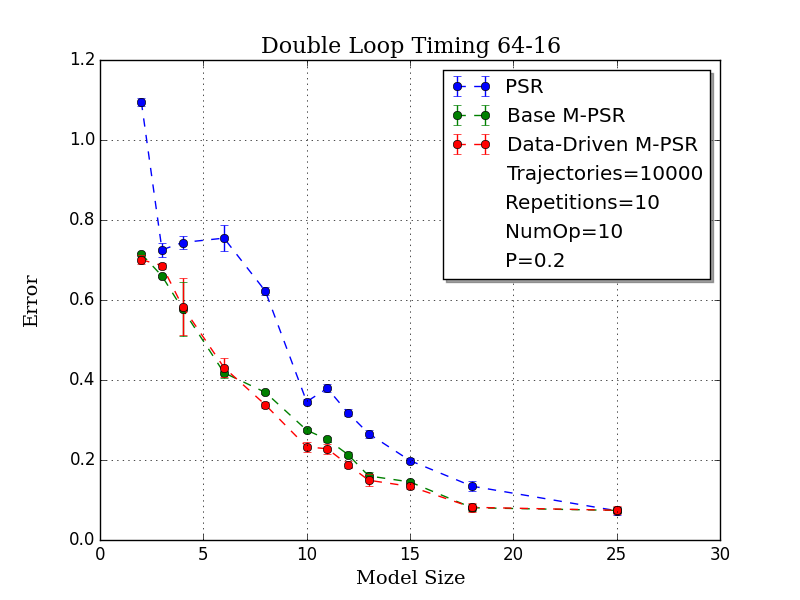
\includegraphics[width=60mm]{uCOREPICS/DL/NoiseInfo.png}
\caption{Noisy Double Loop 64-16\label{overflow}}
\end{figure}

\subsection{Loop Lengths}

In Figure 4, we plot the results of a 47-27 labyrinth, where observations will not be as compactly expressed from the Base M-PSR. Again, M-PSRs outperform the standard PSR for reduced model sizes. In addition we see that the Data-Driven M-PSR does better than the Base M-PSR.

\begin{figure}[ht!]
\centering
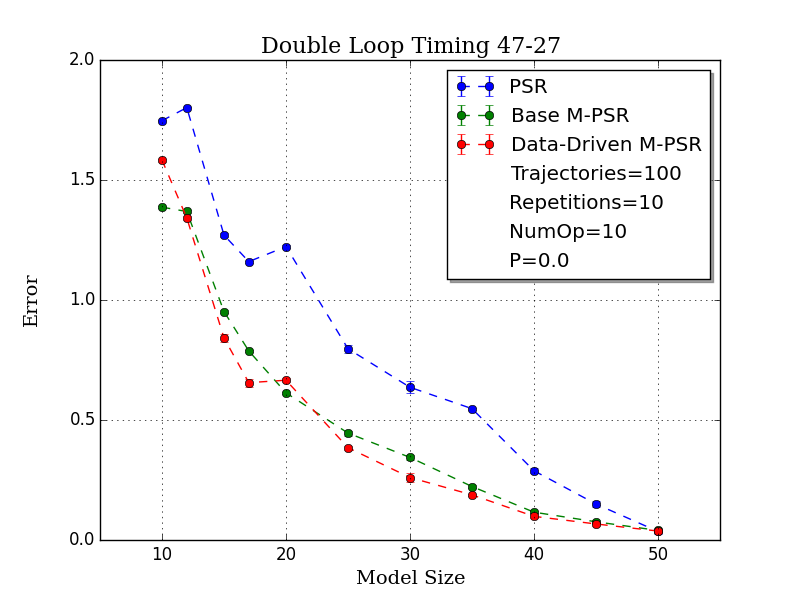
\includegraphics[width=60mm]{uCOREPICS/DL/47-27-10000.png}
\caption{High Data Double Loop 47-27\label{overflow}}
\end{figure}

\subsection{Choice of K for Base M-PSRs}

In Figure 5, we plot performance of Base M-PSRs with different values of L. We note that larger values of K have better performance up to K=7.

\begin{figure}[ht!]
\centering
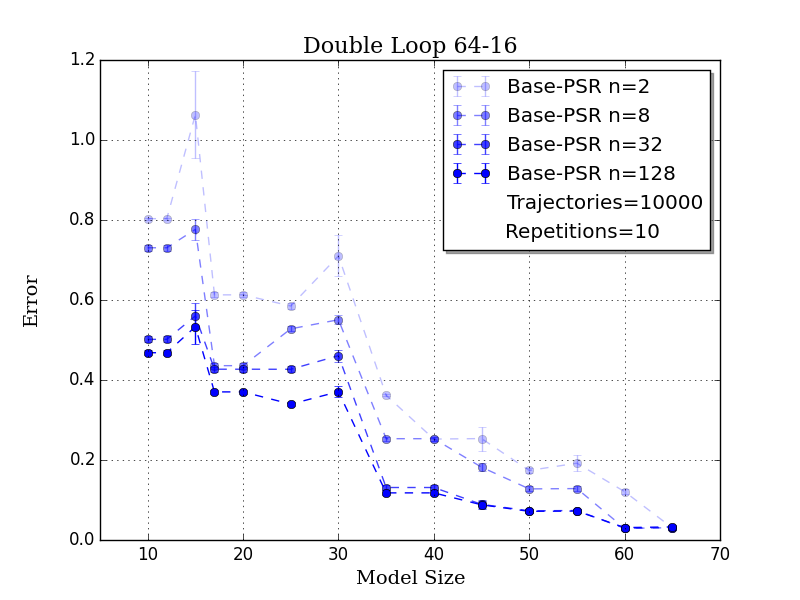
\includegraphics[width=60mm]{uCOREPICS/DL/basePows.png}
\caption{Double Loop 64-16\label{overflow}}
\end{figure}

\subsection{Varying NumOps}

In Figure 6, we look at how the varying the number of multi-step transition operators affects performance for the 64-16 double loop. In this environment, a higher number of operators improves performance up until about 20 operators. Here the most important operators seem to be: $\{a,a^{8},a^{24},a^{32},a^{72}\}$ which are closely tied to the environment's structure.

\begin{figure}[ht!]
\centering
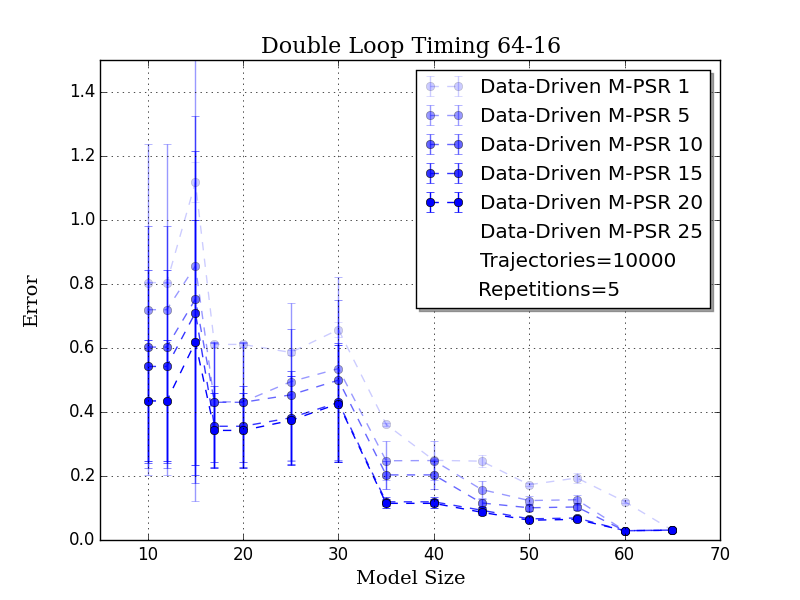
\includegraphics[width=60mm]{uCOREPICS/DL/numOpsTiming.png}
\caption{Varying NumOps\label{overflow}}
\end{figure} 

\section{Large Labyrinth Timing}

We proceed to work with a labyrinth environment similar to a Pacman game. A graphical representation of this labyrinth is available in the appendix. Transitions to new states occur with equal probability. The weight $w(u,v)$ between states u and v corresponds to the number of time steps from u to v. We add an additional parameter sF: stretch factor, which scales all of the weights in the graph. 

\subsection{Number of Trajectories}

In Figure 7,8 we vary the number of observations used for learning. M-PSRs outperform the traditional PSR regardless of the amount of data. Secondly, as expected, the performance of all models is worse for less data.

\begin{figure}[ht!]
\centering
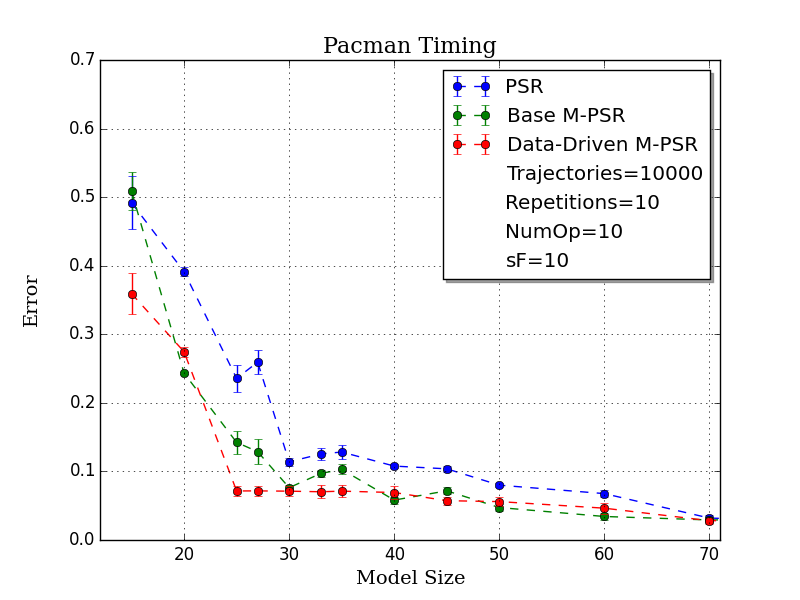
\includegraphics[width=60mm]{uCOREPICS/Pacman/Pacman10k.png}
\caption{High Data Pacman Labyrinth\label{overflow}}
\end{figure}

\begin{figure}[ht!]
\centering
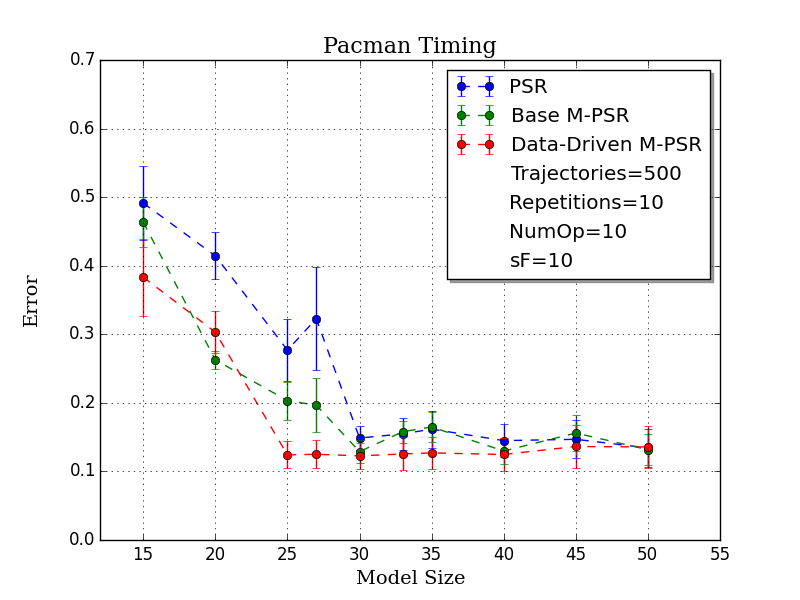
\includegraphics[width=60mm]{uCOREPICS/Pacman/Pacman500.png}
\caption{Low Data Pacman Labyrinth\label{overflow}}
\end{figure}

\subsection{Stretch Factor: sF}

In Figures 7,9 and 10 we vary the stretch factor parameter with a fixed dataset. We find that a higher values of sF allow for increased improvement of the M-PSR relative to the performance of the standard PSR.

\begin{figure}[ht!]
\centering
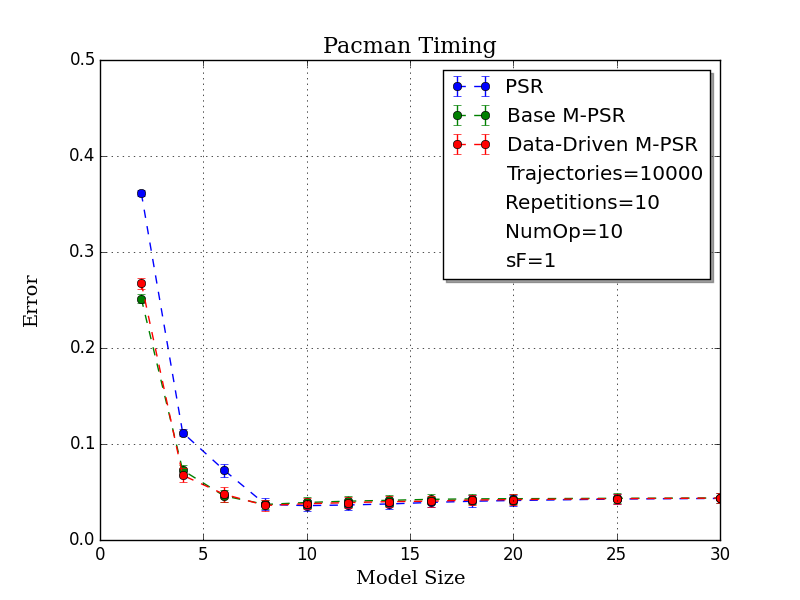
\includegraphics[width=60mm]{uCOREPICS/Pacman/PacmanSF=1.png}
\caption{Stretch Factor: 1\label{overflow}}
\end{figure}

\begin{figure}[ht!]
\centering
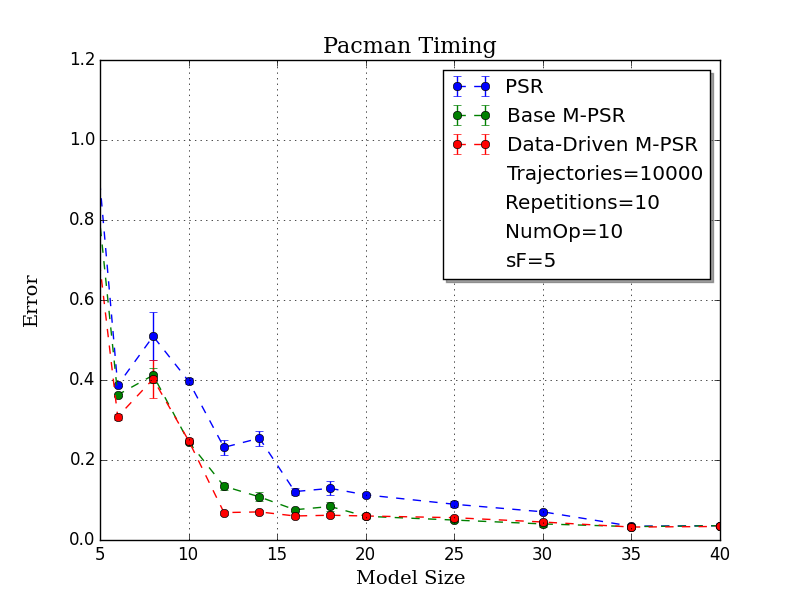
\includegraphics[width=60mm]{uCOREPICS/Pacman/PacmanSF=5.png}
\caption{Stretch Factor: 5\label{overflow}}
\end{figure}

\section{Multiple Observations: Coloured Loops}

We now move to the multiple observation case. We construct a Double Loop environment where loop1 is green with $l_1=27$ and loop2 is blue with $l_2=17$. We fix the length of observations to be:
\begin{equation*}
TrajectoryLength := (l_1 + l_2)*3
\end{equation*} 

We build empirical estimates for the hankel matrix as follows:
\begin{equation*}
 f(x)=\dfrac{count([s \in Obs, s=x])}{count([s \in Obs, |s| \geq x])}
\end{equation*}  
This means that the PSRs will compute the probability of x occurring as a prefix.

\subsection{Number of Trajectories}

As for the timing case, we vary the amount of data to learn PSRS/M-PSRs in Figures 11 and 12. Once again we find M-PSRs perform far better, especially the Data-Driven M-PSR. This makes sense as when complexity in observations increases only custom M-PSRs will express transitions compactly.

\begin{figure}[ht!]
\centering
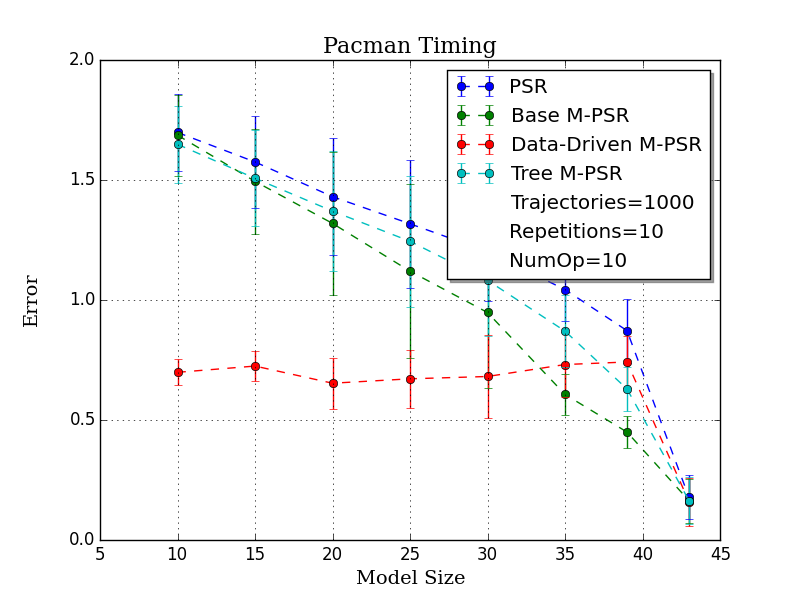
\includegraphics[width=60mm]{uCOREPICS/DLMO/MO_1k.png}
\caption{High Data Colored Loops 27-17\label{overflow}}
\end{figure}

\begin{figure}[ht!]
\centering
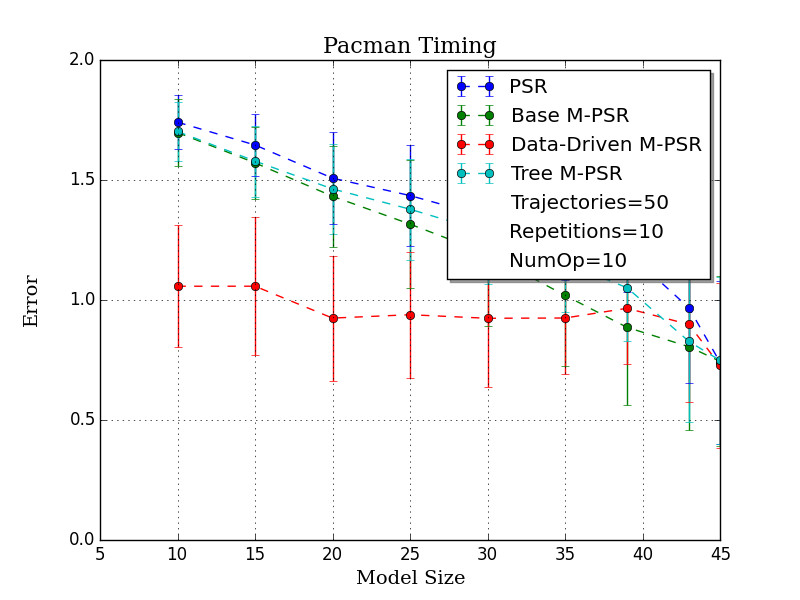
\includegraphics[width=60mm]{uCOREPICS/DLMO/MO_50.png}
\caption{Low Data Colored Loops 27-17\label{overflow}}
\end{figure}

\subsection{Varying NumOps}

In Figure 13, we vary the number of multi-step transition operators learned. Here the important operators seem to be $\{g,b,g^{27},b^{17}\}$ which reflects the structure of the environment.

\begin{figure}[ht!]
\centering
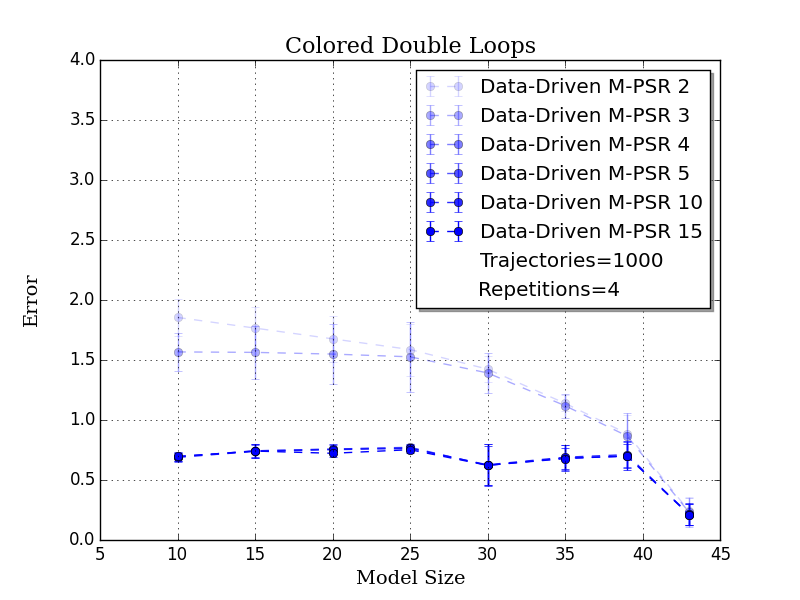
\includegraphics[width=60mm]{uCOREPICS/DLMO/numOpComparison.png}
\caption{Varying NumOps\label{overflow}}
\end{figure}
